\begin{figure}
\centering

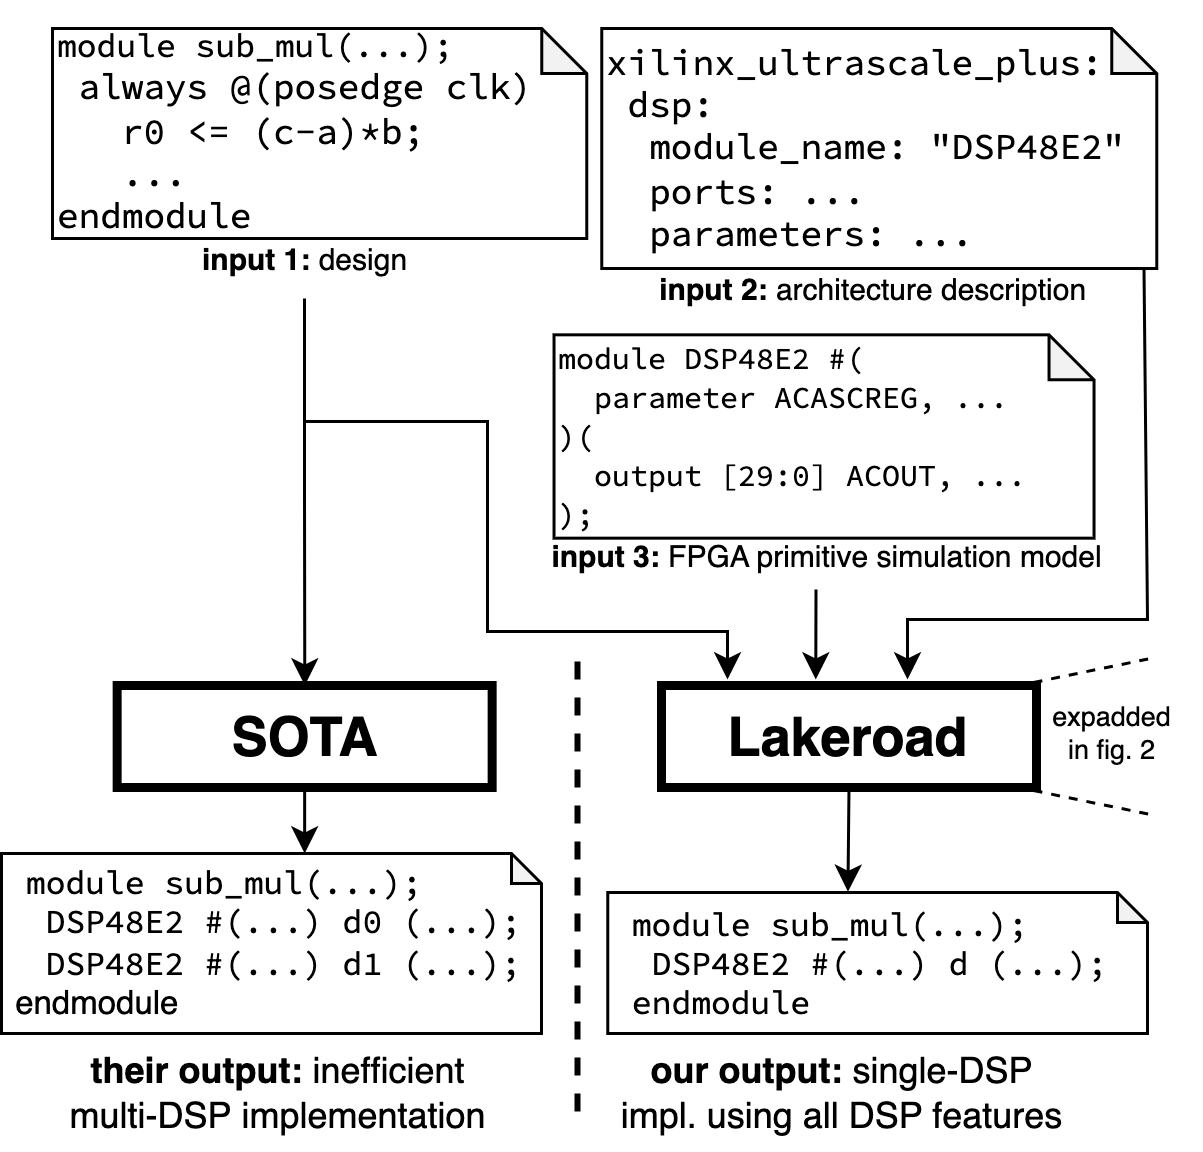
\includegraphics[width=0.91\columnwidth]{assets/lakeroad-firstpage.drawio.png}

% \vspace{3mm}
% \resizebox{0.4\textwidth}{!}{
% \begin{tabular}{cc|c|c}
% Design& \# Stages &  SOTA& \lr \\ \hline
% \texttt{((d+a)*b)|c}& 1 &2 DSP, 18 LUT & 1 DSP  \\
% \texttt{((d+a)*b)\textasciicircum{}c} & 1 & 2 DSP, 18 LUT  & 1 DSP \\
% \texttt{((d-a)*b)|c} & 2 & 2 DSP, 18 LUT & 1 DSP \\
% \texttt{((d-a)*b)\textasciicircum{}c} &  2          & 2 DSP, 18 LUT & 1 DSP \\
% \texttt{((d+a)*b)\&c}& 2 & 2 DSP, 18 LUT & 1 DSP \\
% \end{tabular}}
\vspace{-3mm}
\caption{
% Mapping a simple design to
%   Xilinx UltraScale+ FPGAs with both
%   the state of the art (SOTA)
%   hardware synthesis tool for Xilinx
%   and \lr.
Even given a simple input
  design (input 1),
  the state-of-the-art (SOTA)
  hardware synthesis tool
  for Xilinx FPGAs
  frequently
  fails to efficiently use 
  programmable primitives
  like DSPs.
\lr,
  on the other hand,
  can utilize all features
  of programmable primitives
  given just a short description
  of an FPGA architecture (input 2)
  and the vendor-provided 
  simulation models
  of the primitive (input 3).\tighten
}
\label{fig:firstpage}

\vspace{-5mm}
\end{figure}


FPGA technology mapping is the process of
  implementing a hardware design expressed in 
  high-level HDL (hardware design language) code
  using the low-level, architecture-specific primitives of 
  the target FPGA.
As FPGAs become increasingly heterogeneous, 
  achieving high performance
  requires hardware synthesis tools 
  that better support mapping to complex, 
  highly configurable primitives 
  like digital signal processors (DSPs).
Current tools
  support DSP mapping via handwritten special-case mapping rules,
  which are laborious to write, error-prone, and often overlook mapping opportunities.
We introduce \lr,
  a principled approach to technology mapping via
  sketch-guided program synthesis.
\lr leverages two techniques---architecture-independent 
  sketch templates and semantics extraction from HDL---to
  provide extensible technology mapping 
  with stronger correctness guarantees
  and higher coverage of 
  % micro-design 
  mapping opportunities
  than state-of-the-art tools.
Across representative microbenchmarks,
  \lr produces
  2--3.5$\times$ the number of optimal mappings
  compared to proprietary state-of-the-art tools
  and
  6--44$\times$ the number of optimal mappings
  compared to popular open-source tools,
  while also providing correctness guarantees
  not given by any other tool.
